\section{Remorque}
\begin{figure}[H]
    \centering
    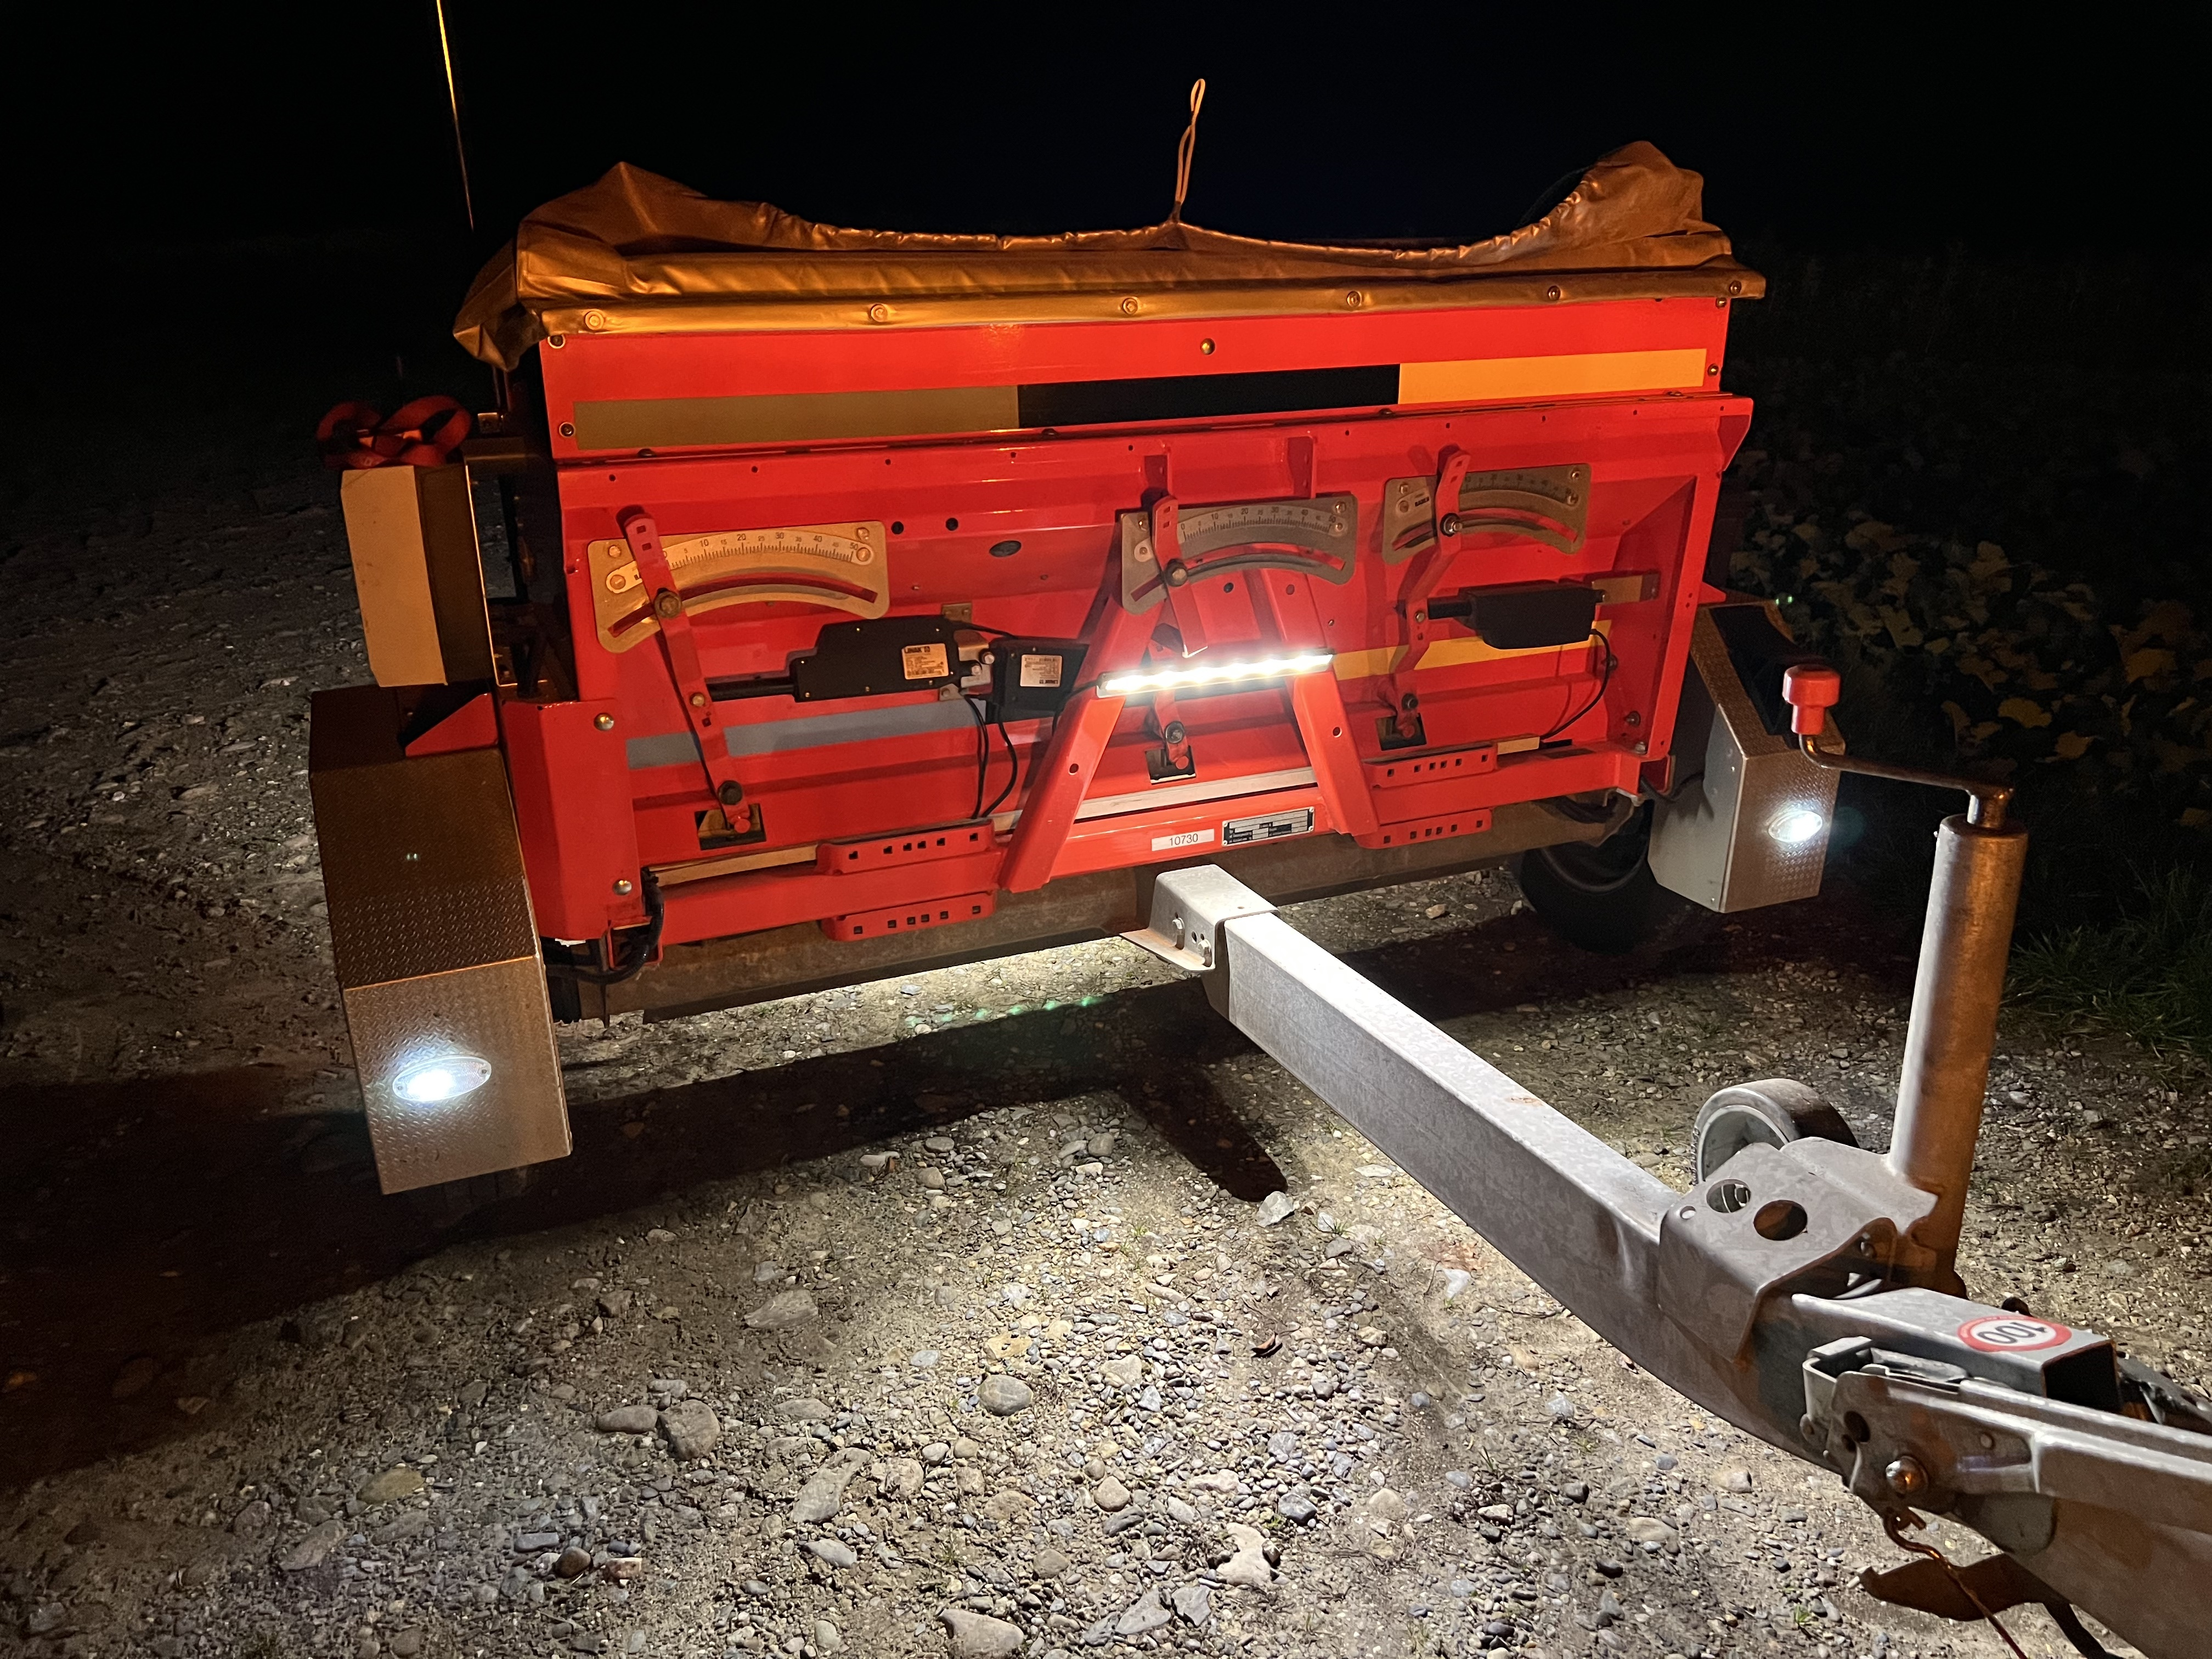
\includegraphics[width=12cm]{assets/figures/remorque.jpeg}
    \caption{Remorque - Vue intérieur}
\end{figure}
\subsection{Caractéristique}
\begin{table}[H]
    \begin{center}
        \caption{Liste de mesure de la remorque}
        \begin{tabular}{|l|l|l|}
            Dimensions                           & Valeurs                   & Commentaire \\ \hline
            Largeur total des semoires           & 1.56\textbf{[m]}          & [1]         \\
            Largeur d'un semoir                  & 520[mm]                   & -           \\
            Barre remorque - l x H               & 70 [mm] x 135[mm]         & -           \\
            Barre remorque - hauteur sol         & 270[mm]                   & -           \\
            Barre remorque - longueur            & 2.5\textbf{[m]}           & -           \\
            Distance sans obstacle depuis semoir & 780[mm]                   & -           \\
            Dimensions télécommande L x l x H    & 133[mm] x 62[mm] x 25[mm] & [2]         \\
            Enfoncement des boutons              & ~3-4[mm]                  & [3]         \\
        \end{tabular}
    \end{center}
\end{table}\\
\begin{enumerate}
    \item{Le champ d'action du semoir est beaucoup plus petit qu'une voie de circulation. En Suisse, une voie d'une route cantonnale mesure entre 3 et 3.5[m].}
    \item{La télécommande n'est pas parfaitement rectangulaire. Le mécanisme d'activation du l'émetteur de la télécommande occupe la partie gauche de la télécommande,
                si une pression est exercéce contre la télécommande, celle-ci ce découple de la commande des semoirs. Il y a également une attache sur la droite de la télécommande.}
    \item{Il y a un "déclique" à atteindre pour actionner les boutons, d'après la mesure qui a été effectuée, il faut une pression de 820 \si{\gram}, ce qui correspond à environ 8 \si{\newton}}.
\end{enumerate}

\begin{figure}[H]
    \centering
    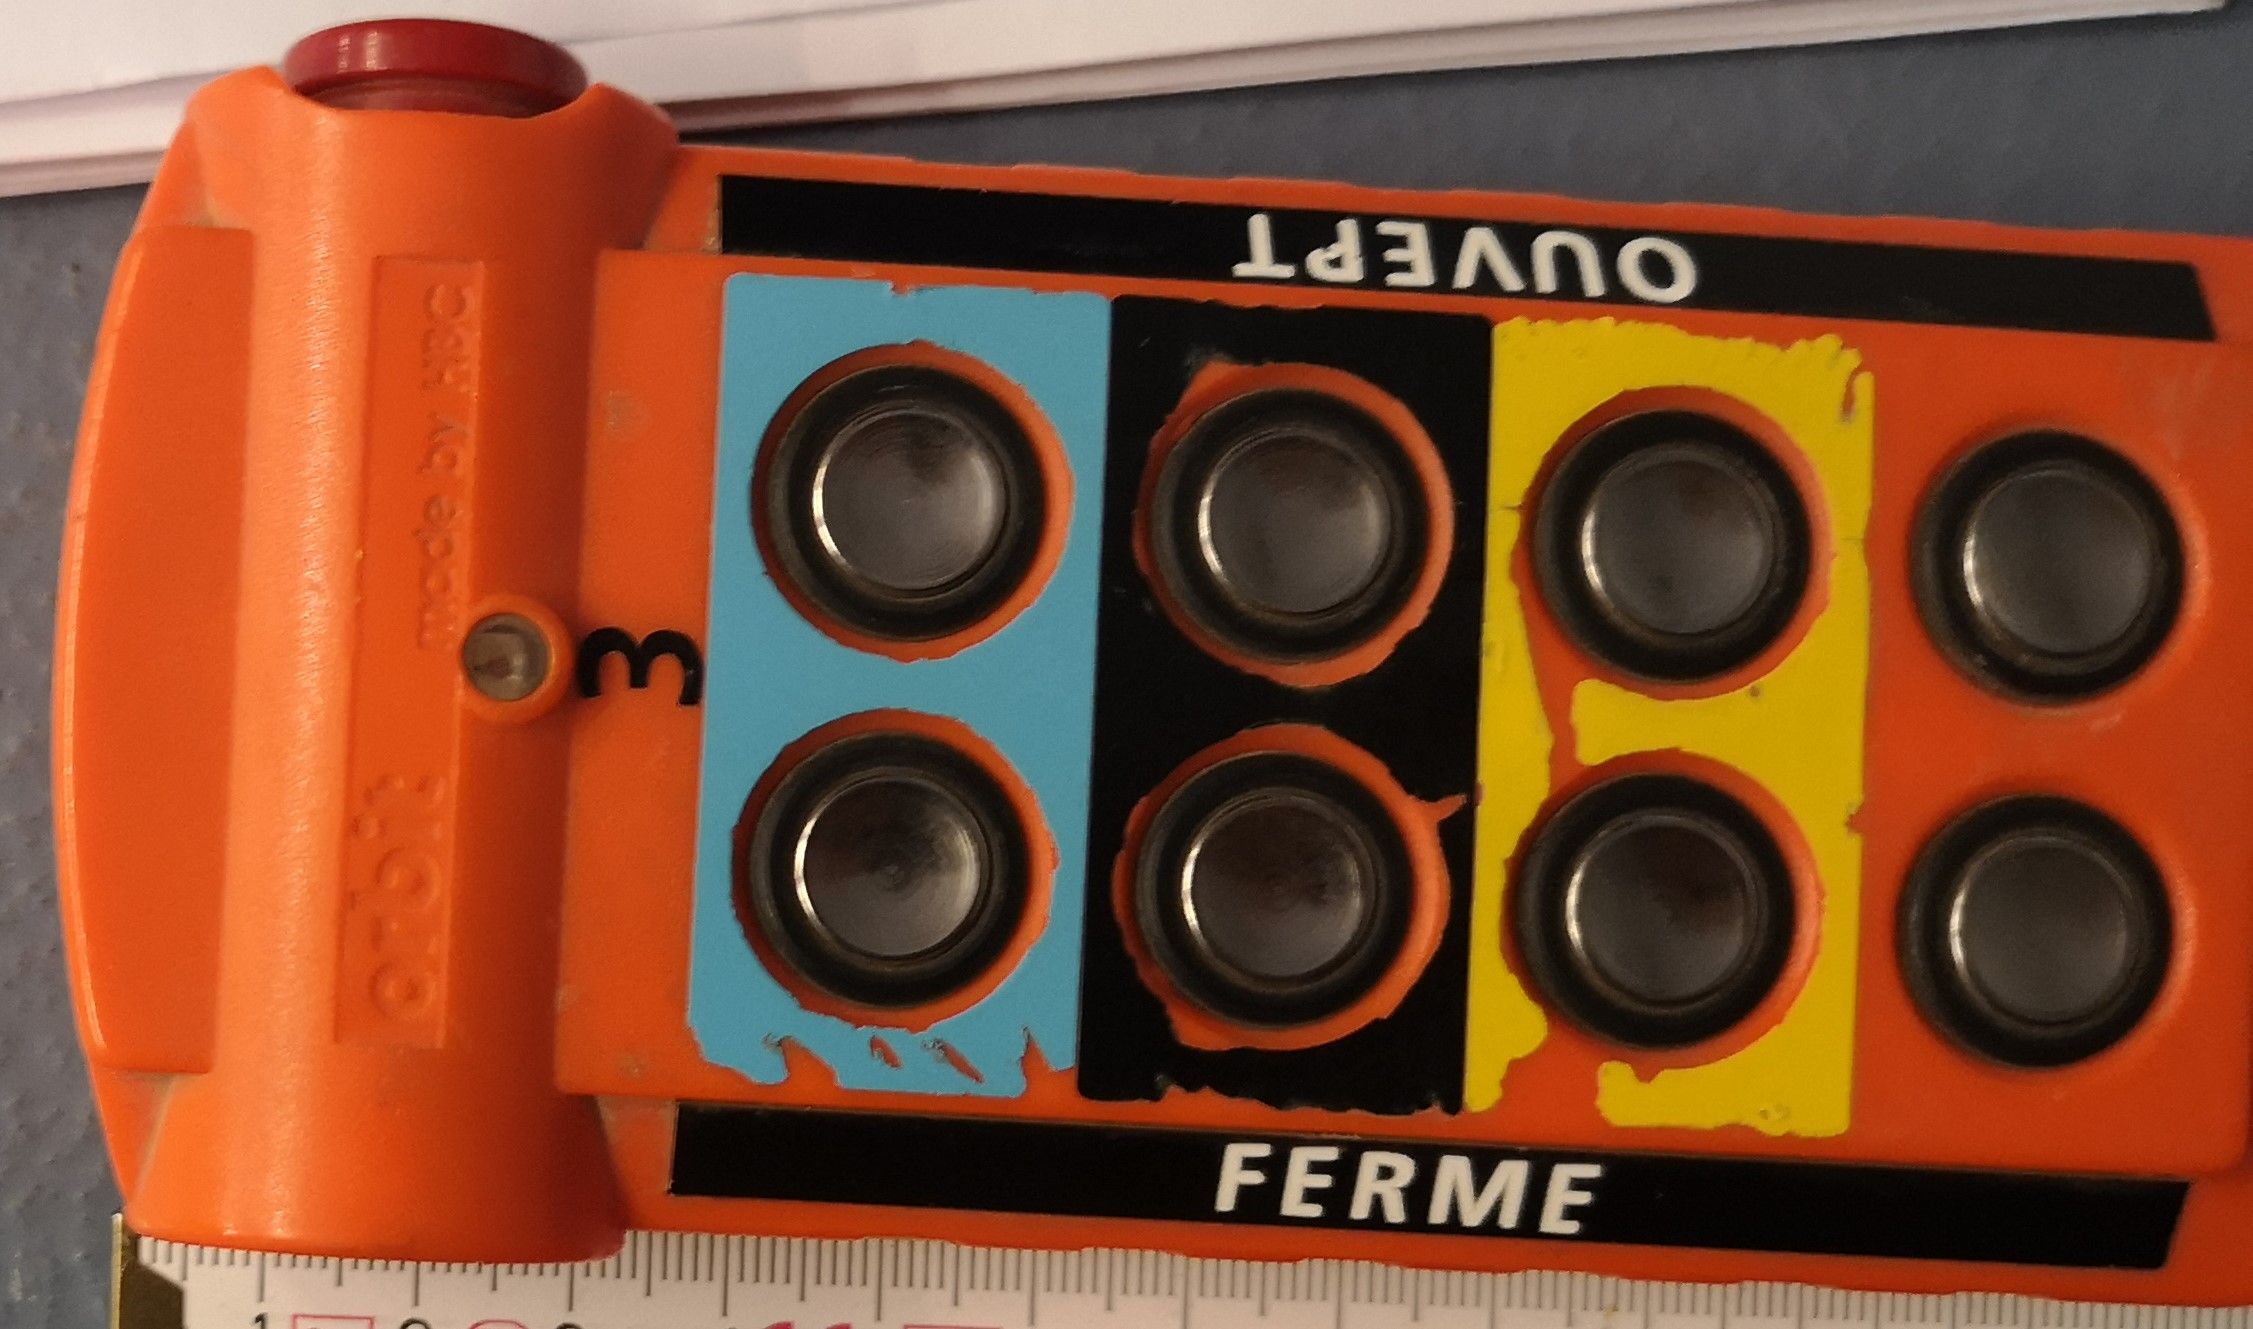
\includegraphics[width=7cm]{assets/figures/telecommande2.jpg}
    \caption{Télécommande - Contrôles des ouvertures}
\end{figure}

\subsection{Alimentation}
Plusieurs sources sont disponibles sur les véhicules tractant la remorque.
\begin{itemize}
    \item{Véhicule 1: 2x prises 13 broches.}
    \item{Véhicule 2: 1x prise 13 broches, 1x prise 7 broches.}
\end{itemize}
A noter que l'installation de base sur la remorque utilise une prise 13 broches.\\
Il est possible d'avoir du 12 [V] à disposition avec une prise 13 broches.

\subsection{Fixation}
\subsubsection{Timon de la remorque}
Une partie du timon (environ 78cm) est totalement libre et permettrait d'accrocher du matériel, par exemple un éclairage et/ou une caméra.
Il faudrait malgré tout une fixation adaptée aux dimensions mentionnées dans le tableau de mesure.
\subsubsection{Supports de la remorque}
Il y a deux supports sur la facade intérieure de la remorque, un de chaque côté du timon.
\begin{figure}[H]
    \centering
    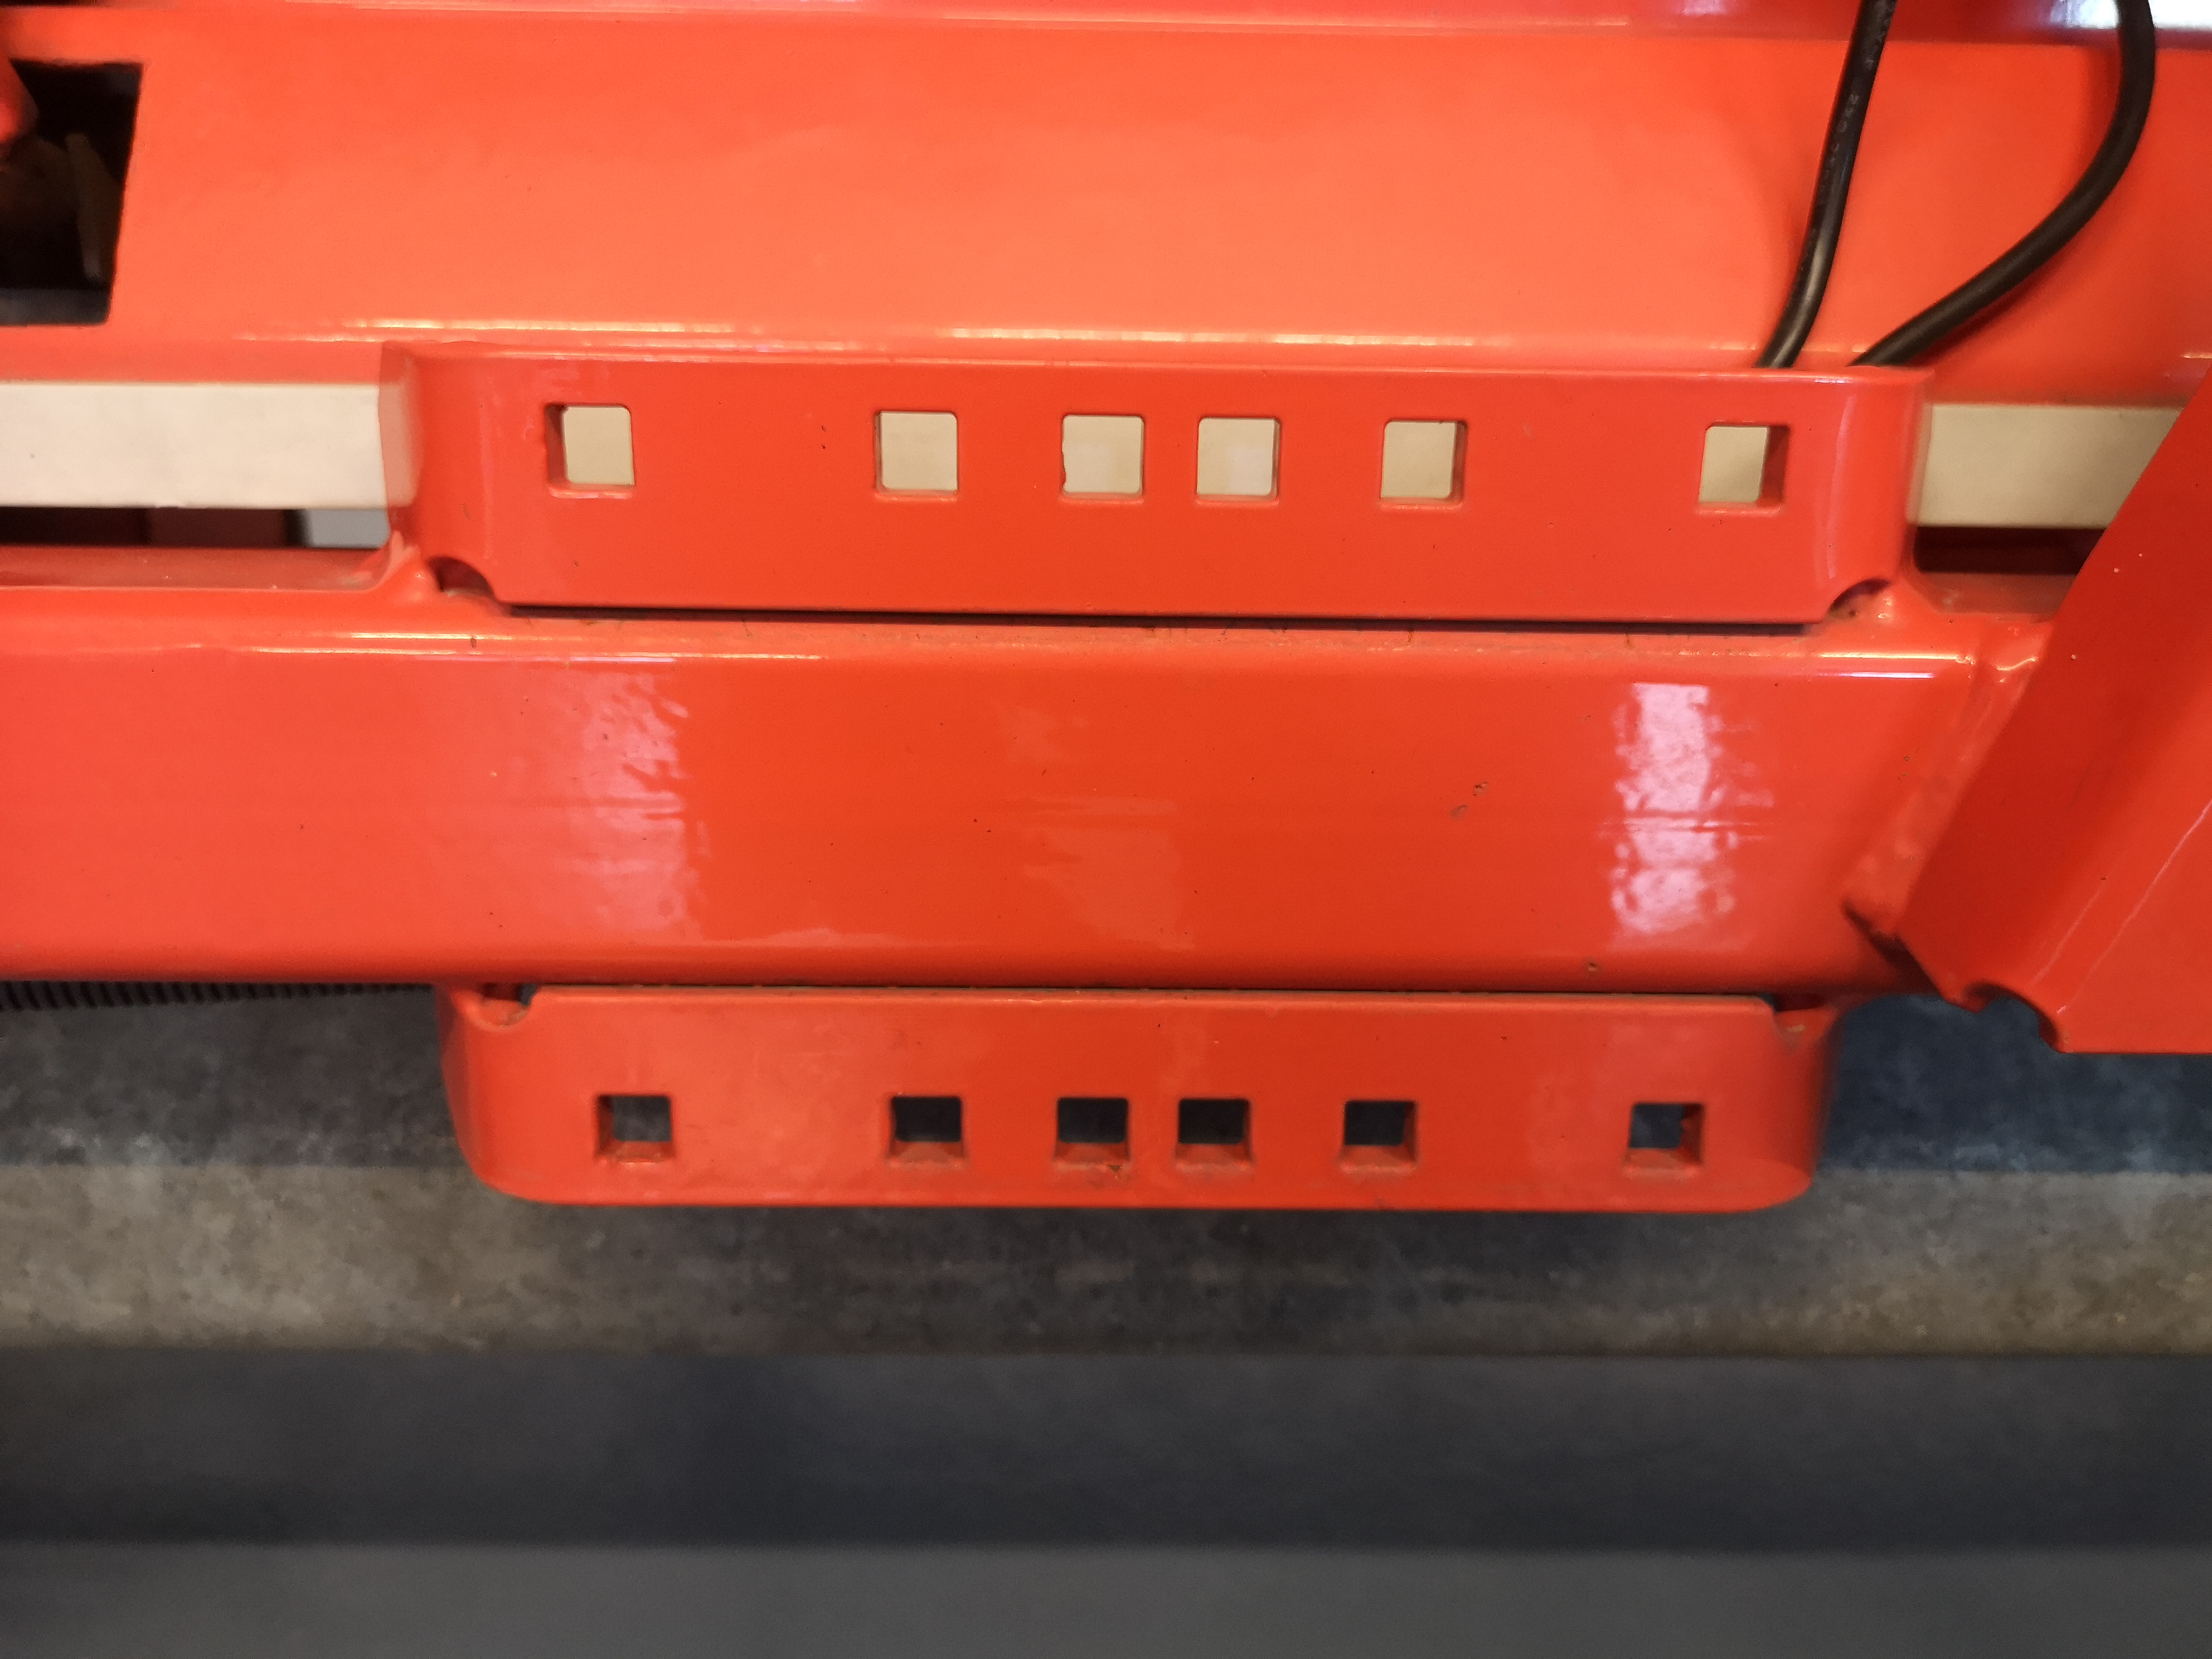
\includegraphics[width=13cm]{assets/figures/support.jpg}
    \caption{Remorque - Support}
\end{figure}

Son emplacement et sa taille pourrait permettre d'y fixer un boitier ou autres éléments relativement facilement.